% Options for packages loaded elsewhere
\PassOptionsToPackage{unicode}{hyperref}
\PassOptionsToPackage{hyphens}{url}
\PassOptionsToPackage{dvipsnames,svgnames*,x11names*}{xcolor}
%
\documentclass[
  ignorenonframetext,
]{beamer}
\usepackage{pgfpages}
\setbeamertemplate{caption}[numbered]
\setbeamertemplate{caption label separator}{: }
\setbeamercolor{caption name}{fg=normal text.fg}
\beamertemplatenavigationsymbolsempty
% Prevent slide breaks in the middle of a paragraph
\widowpenalties 1 10000
\raggedbottom
\setbeamertemplate{part page}{
  \centering
  \begin{beamercolorbox}[sep=16pt,center]{part title}
    \usebeamerfont{part title}\insertpart\par
  \end{beamercolorbox}
}
\setbeamertemplate{section page}{
  \centering
  \begin{beamercolorbox}[sep=12pt,center]{part title}
    \usebeamerfont{section title}\insertsection\par
  \end{beamercolorbox}
}
\setbeamertemplate{subsection page}{
  \centering
  \begin{beamercolorbox}[sep=8pt,center]{part title}
    \usebeamerfont{subsection title}\insertsubsection\par
  \end{beamercolorbox}
}
\AtBeginPart{
  \frame{\partpage}
}
\AtBeginSection{
  \ifbibliography
  \else
    \frame{\sectionpage}
  \fi
}
\AtBeginSubsection{
  \frame{\subsectionpage}
}
\usepackage{lmodern}
\usepackage{amssymb,amsmath}
\usepackage{ifxetex,ifluatex}
\ifnum 0\ifxetex 1\fi\ifluatex 1\fi=0 % if pdftex
  \usepackage[T1]{fontenc}
  \usepackage[utf8]{inputenc}
  \usepackage{textcomp} % provide euro and other symbols
\else % if luatex or xetex
  \usepackage{unicode-math}
  \defaultfontfeatures{Scale=MatchLowercase}
  \defaultfontfeatures[\rmfamily]{Ligatures=TeX,Scale=1}
\fi
% Use upquote if available, for straight quotes in verbatim environments
\IfFileExists{upquote.sty}{\usepackage{upquote}}{}
\IfFileExists{microtype.sty}{% use microtype if available
  \usepackage[]{microtype}
  \UseMicrotypeSet[protrusion]{basicmath} % disable protrusion for tt fonts
}{}
\makeatletter
\@ifundefined{KOMAClassName}{% if non-KOMA class
  \IfFileExists{parskip.sty}{%
    \usepackage{parskip}
  }{% else
    \setlength{\parindent}{0pt}
    \setlength{\parskip}{6pt plus 2pt minus 1pt}}
}{% if KOMA class
  \KOMAoptions{parskip=half}}
\makeatother
\usepackage{xcolor}
\IfFileExists{xurl.sty}{\usepackage{xurl}}{} % add URL line breaks if available
\IfFileExists{bookmark.sty}{\usepackage{bookmark}}{\usepackage{hyperref}}
\hypersetup{
  pdftitle={Review of Introductory Statistics},
  pdfauthor={Zack Treisman},
  colorlinks=true,
  linkcolor=Maroon,
  filecolor=Maroon,
  citecolor=blue,
  urlcolor=Blue,
  pdfcreator={LaTeX via pandoc}}
\urlstyle{same} % disable monospaced font for URLs
\newif\ifbibliography
\usepackage{color}
\usepackage{fancyvrb}
\newcommand{\VerbBar}{|}
\newcommand{\VERB}{\Verb[commandchars=\\\{\}]}
\DefineVerbatimEnvironment{Highlighting}{Verbatim}{commandchars=\\\{\}}
% Add ',fontsize=\small' for more characters per line
\usepackage{framed}
\definecolor{shadecolor}{RGB}{248,248,248}
\newenvironment{Shaded}{\begin{snugshade}}{\end{snugshade}}
\newcommand{\AlertTok}[1]{\textcolor[rgb]{0.94,0.16,0.16}{#1}}
\newcommand{\AnnotationTok}[1]{\textcolor[rgb]{0.56,0.35,0.01}{\textbf{\textit{#1}}}}
\newcommand{\AttributeTok}[1]{\textcolor[rgb]{0.77,0.63,0.00}{#1}}
\newcommand{\BaseNTok}[1]{\textcolor[rgb]{0.00,0.00,0.81}{#1}}
\newcommand{\BuiltInTok}[1]{#1}
\newcommand{\CharTok}[1]{\textcolor[rgb]{0.31,0.60,0.02}{#1}}
\newcommand{\CommentTok}[1]{\textcolor[rgb]{0.56,0.35,0.01}{\textit{#1}}}
\newcommand{\CommentVarTok}[1]{\textcolor[rgb]{0.56,0.35,0.01}{\textbf{\textit{#1}}}}
\newcommand{\ConstantTok}[1]{\textcolor[rgb]{0.00,0.00,0.00}{#1}}
\newcommand{\ControlFlowTok}[1]{\textcolor[rgb]{0.13,0.29,0.53}{\textbf{#1}}}
\newcommand{\DataTypeTok}[1]{\textcolor[rgb]{0.13,0.29,0.53}{#1}}
\newcommand{\DecValTok}[1]{\textcolor[rgb]{0.00,0.00,0.81}{#1}}
\newcommand{\DocumentationTok}[1]{\textcolor[rgb]{0.56,0.35,0.01}{\textbf{\textit{#1}}}}
\newcommand{\ErrorTok}[1]{\textcolor[rgb]{0.64,0.00,0.00}{\textbf{#1}}}
\newcommand{\ExtensionTok}[1]{#1}
\newcommand{\FloatTok}[1]{\textcolor[rgb]{0.00,0.00,0.81}{#1}}
\newcommand{\FunctionTok}[1]{\textcolor[rgb]{0.00,0.00,0.00}{#1}}
\newcommand{\ImportTok}[1]{#1}
\newcommand{\InformationTok}[1]{\textcolor[rgb]{0.56,0.35,0.01}{\textbf{\textit{#1}}}}
\newcommand{\KeywordTok}[1]{\textcolor[rgb]{0.13,0.29,0.53}{\textbf{#1}}}
\newcommand{\NormalTok}[1]{#1}
\newcommand{\OperatorTok}[1]{\textcolor[rgb]{0.81,0.36,0.00}{\textbf{#1}}}
\newcommand{\OtherTok}[1]{\textcolor[rgb]{0.56,0.35,0.01}{#1}}
\newcommand{\PreprocessorTok}[1]{\textcolor[rgb]{0.56,0.35,0.01}{\textit{#1}}}
\newcommand{\RegionMarkerTok}[1]{#1}
\newcommand{\SpecialCharTok}[1]{\textcolor[rgb]{0.00,0.00,0.00}{#1}}
\newcommand{\SpecialStringTok}[1]{\textcolor[rgb]{0.31,0.60,0.02}{#1}}
\newcommand{\StringTok}[1]{\textcolor[rgb]{0.31,0.60,0.02}{#1}}
\newcommand{\VariableTok}[1]{\textcolor[rgb]{0.00,0.00,0.00}{#1}}
\newcommand{\VerbatimStringTok}[1]{\textcolor[rgb]{0.31,0.60,0.02}{#1}}
\newcommand{\WarningTok}[1]{\textcolor[rgb]{0.56,0.35,0.01}{\textbf{\textit{#1}}}}
\usepackage{graphicx,grffile}
\makeatletter
\def\maxwidth{\ifdim\Gin@nat@width>\linewidth\linewidth\else\Gin@nat@width\fi}
\def\maxheight{\ifdim\Gin@nat@height>\textheight\textheight\else\Gin@nat@height\fi}
\makeatother
% Scale images if necessary, so that they will not overflow the page
% margins by default, and it is still possible to overwrite the defaults
% using explicit options in \includegraphics[width, height, ...]{}
\setkeys{Gin}{width=\maxwidth,height=\maxheight,keepaspectratio}
% Set default figure placement to htbp
\makeatletter
\def\fps@figure{htbp}
\makeatother
\setlength{\emergencystretch}{3em} % prevent overfull lines
\providecommand{\tightlist}{%
  \setlength{\itemsep}{0pt}\setlength{\parskip}{0pt}}
\setcounter{secnumdepth}{-\maxdimen} % remove section numbering

\pgfdeclareimage[width=3.5cm]{mcslogo}{../western_logo_hor_MCS_3C_pos.pdf}
\pgfdeclareimage[width=1cm]{ccbysa}{../ccbysa88x31.png}
\titlegraphic{\href{http://creativecommons.org/licenses/by-sa/4.0/}{\pgfuseimage{ccbysa}}
\hfill
\href{https://western.edu/program/mathematics/}{\pgfuseimage{mcslogo}}}
%\usecolortheme{wcu}
%\institute{Western Colorado University}
%\setbeamertemplate{navigation symbols}{}

\title{Review of Introductory Statistics}
\author{Zack Treisman}
\date{Spring 2021}

\begin{document}
\frame{\titlepage}

\begin{frame}[fragile]{Data}
\protect\hypertarget{data}{}

An \textbf{observation} is a single unit. A \textbf{variable} is a
measurement made on that unit

\begin{itemize}
\tightlist
\item
  Record observations as \textbf{rows} and variables in
  \textbf{columns}.\\
\item
  Variables can be \textbf{categorical} or \textbf{numerical}.

  \begin{itemize}
  \tightlist
  \item
    Categorical variables can be \textbf{binary} or not,
    \textbf{ordered} or not.
  \item
    Numerical variables can be \textbf{discrete} or \textbf{continuous}.
  \end{itemize}
\item
  Dates, times and locations merit special consideration.
\item
  Vocabulary is not universal: Factor, case, treatment \ldots
\end{itemize}

\begin{Shaded}
\begin{Highlighting}[]
\KeywordTok{head}\NormalTok{(Sitka) }\CommentTok{# from package MASS}
\end{Highlighting}
\end{Shaded}

\begin{verbatim}
##   size Time tree treat
## 1 4.51  152    1 ozone
## 2 4.98  174    1 ozone
## 3 5.41  201    1 ozone
## 4 5.90  227    1 ozone
## 5 6.15  258    1 ozone
## 6 4.24  152    2 ozone
\end{verbatim}

\end{frame}

\begin{frame}[fragile]{Distributions}
\protect\hypertarget{distributions}{}

The \textbf{distribution} of a variable is a measure of how often it
takes each possible value.

\begin{itemize}
\tightlist
\item
  The distribution of a categorical variable is a list of the percentage
  of observations in each category.
\end{itemize}

\begin{Shaded}
\begin{Highlighting}[]
\KeywordTok{table}\NormalTok{(Sitka}\OperatorTok{$}\NormalTok{treat)}\OperatorTok{/}\KeywordTok{length}\NormalTok{(Sitka}\OperatorTok{$}\NormalTok{treat)}
\end{Highlighting}
\end{Shaded}

\begin{verbatim}
## 
##   control     ozone 
## 0.3164557 0.6835443
\end{verbatim}

\end{frame}

\begin{frame}[fragile]{Distributions}
\protect\hypertarget{distributions-1}{}

\begin{itemize}
\tightlist
\item
  Picture the distribution of a numerical variable with a histogram,
  boxplot or density estimate.
\end{itemize}

\begin{Shaded}
\begin{Highlighting}[]
\KeywordTok{hist}\NormalTok{(Sitka}\OperatorTok{$}\NormalTok{size)}
\end{Highlighting}
\end{Shaded}

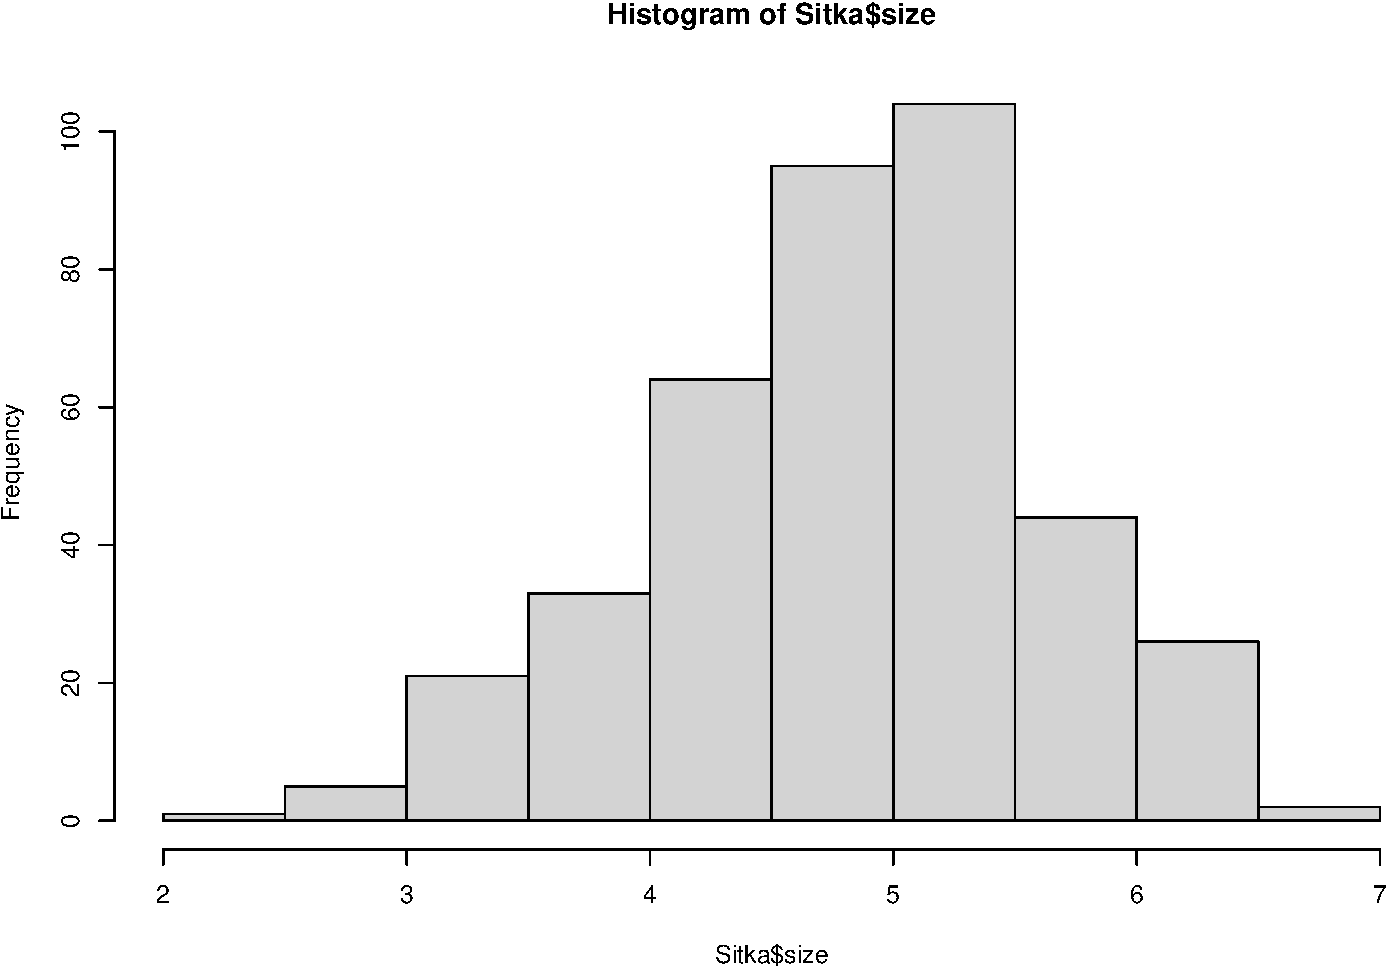
\includegraphics[height=0.5\textheight]{review_files/figure-beamer/unnamed-chunk-3-1}

\begin{itemize}
\tightlist
\item
  Shape: center, spread, skew, kurtosis
\end{itemize}

\end{frame}

\begin{frame}[fragile]{Numerical summaries}
\protect\hypertarget{numerical-summaries}{}

\begin{Shaded}
\begin{Highlighting}[]
\KeywordTok{summary}\NormalTok{(Sitka}\OperatorTok{$}\NormalTok{size)}
\end{Highlighting}
\end{Shaded}

\begin{verbatim}
##    Min. 1st Qu.  Median    Mean 3rd Qu.    Max. 
##   2.230   4.345   4.900   4.841   5.400   6.630
\end{verbatim}

\begin{Shaded}
\begin{Highlighting}[]
\KeywordTok{quantile}\NormalTok{(Sitka}\OperatorTok{$}\NormalTok{size, }\KeywordTok{c}\NormalTok{(}\FloatTok{0.025}\NormalTok{,}\FloatTok{0.975}\NormalTok{))}
\end{Highlighting}
\end{Shaded}

\begin{verbatim}
##   2.5%  97.5% 
## 3.2370 6.2815
\end{verbatim}

\begin{Shaded}
\begin{Highlighting}[]
\KeywordTok{sd}\NormalTok{(Sitka}\OperatorTok{$}\NormalTok{size)}
\end{Highlighting}
\end{Shaded}

\begin{verbatim}
## [1] 0.7982084
\end{verbatim}

\begin{Shaded}
\begin{Highlighting}[]
\KeywordTok{var}\NormalTok{(Sitka}\OperatorTok{$}\NormalTok{size)}
\end{Highlighting}
\end{Shaded}

\begin{verbatim}
## [1] 0.6371367
\end{verbatim}

\begin{Shaded}
\begin{Highlighting}[]
\KeywordTok{IQR}\NormalTok{(Sitka}\OperatorTok{$}\NormalTok{size)}
\end{Highlighting}
\end{Shaded}

\begin{verbatim}
## [1] 1.055
\end{verbatim}

\end{frame}

\begin{frame}{Common distributions}
\protect\hypertarget{common-distributions}{}

\begin{itemize}
\tightlist
\item
  Normal distribution

  \begin{itemize}
  \tightlist
  \item
    The sum of many independent effects tends to be normal.
  \item
    Formula that you never use:
    \(\displaystyle N(\mu,\sigma^2)(x)=\frac{1}{\sigma\sqrt{2 \pi}}e^{-\frac{1}{2}\left(\frac{x-\mu}{\sigma}\right)^2}\)
  \item
    Observations on disparate scales can be standardized with z scores:
    \(\displaystyle z=\frac{x-\mu}{\sigma}\)
  \end{itemize}
\end{itemize}

\medskip

\begin{itemize}
\tightlist
\item
  Other distributions from Intro Stats

  \begin{itemize}
  \tightlist
  \item
    t - Like the normal distribution, but adjusted for small samples.
  \item
    \(\chi^2\) - Sum of squared standard normals.
  \item
    F - Similar to \(\chi^2\), used in ANOVA.
  \item
    Binomial - How many successes in \(n\) trials?
  \item
    Poisson - Count of discrete events in fixed time or space.
  \item
    \ldots
  \end{itemize}
\end{itemize}

\end{frame}

\begin{frame}[fragile]{Inference}
\protect\hypertarget{inference}{}

\begin{itemize}
\tightlist
\item
  Confidence intervals
\item
  Hypothesis tests

  \begin{itemize}
  \tightlist
  \item
    p(robability)-values
  \item
    Null and alternate hypotheses
  \item
    t-tests, ANOVA, \(\chi^2\) tests
  \end{itemize}
\end{itemize}

\footnotesize

\begin{Shaded}
\begin{Highlighting}[]
\KeywordTok{t.test}\NormalTok{(size}\OperatorTok{~}\NormalTok{treat, }\DataTypeTok{data =}\NormalTok{ Sitka)}
\end{Highlighting}
\end{Shaded}

\begin{verbatim}
## 
##  Welch Two Sample t-test
## 
## data:  size by treat
## t = 2.3163, df = 209.44, p-value = 0.02151
## alternative hypothesis: true difference in means is not equal to 0
## 95 percent confidence interval:
##  0.03144833 0.39086574
## sample estimates:
## mean in group control   mean in group ozone 
##              4.985120              4.773963
\end{verbatim}

\normalsize

\end{frame}

\begin{frame}[fragile]{Always plot your data!}
\protect\hypertarget{always-plot-your-data}{}

\begin{Shaded}
\begin{Highlighting}[]
\KeywordTok{boxplot}\NormalTok{(size}\OperatorTok{~}\NormalTok{treat, }\DataTypeTok{data =}\NormalTok{ Sitka)}
\end{Highlighting}
\end{Shaded}

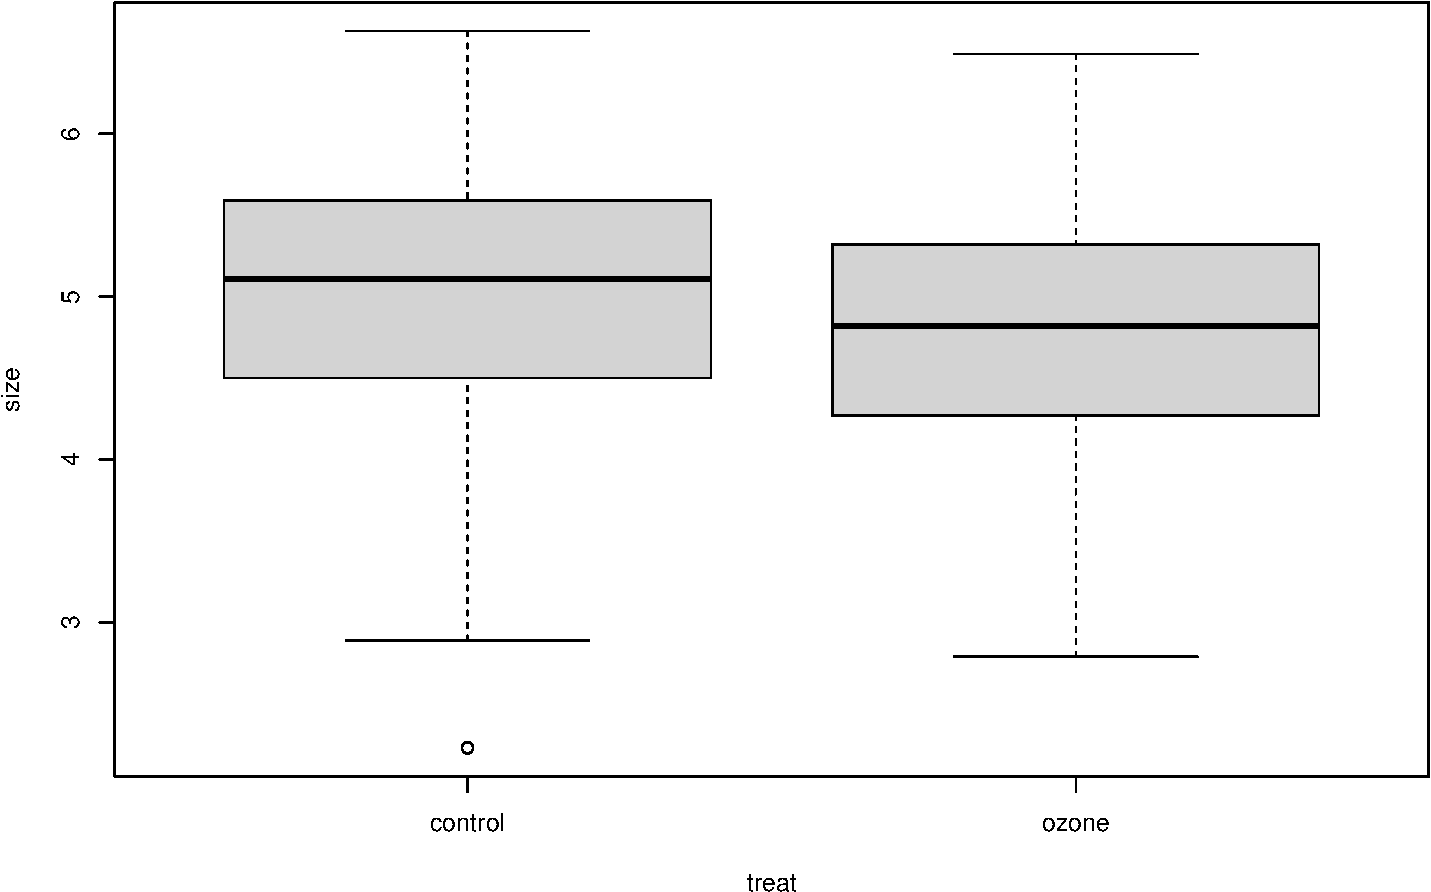
\includegraphics{review_files/figure-beamer/unnamed-chunk-10-1.pdf}

\end{frame}

\begin{frame}[fragile]{Linear models}
\protect\hypertarget{linear-models}{}

\begin{itemize}
\tightlist
\item
  Slope and intercept parameters
\item
  Correlation
\item
  Residuals
\item
  Inference
\end{itemize}

\scriptsize

\begin{Shaded}
\begin{Highlighting}[]
\KeywordTok{summary}\NormalTok{(}\KeywordTok{lm}\NormalTok{(size}\OperatorTok{~}\NormalTok{Time, }\DataTypeTok{data =}\NormalTok{ Sitka))}
\end{Highlighting}
\end{Shaded}

\begin{verbatim}
## 
## Call:
## lm(formula = size ~ Time, data = Sitka)
## 
## Residuals:
##      Min       1Q   Median       3Q      Max 
## -2.02610 -0.37956  0.06948  0.41669  1.30948 
## 
## Coefficients:
##              Estimate Std. Error t value Pr(>|t|)    
## (Intercept) 2.2732443  0.1768643   12.85   <2e-16 ***
## Time        0.0126855  0.0008592   14.77   <2e-16 ***
## ---
## Signif. codes:  0 '***' 0.001 '**' 0.01 '*' 0.05 '.' 0.1 ' ' 1
## 
## Residual standard error: 0.641 on 393 degrees of freedom
## Multiple R-squared:  0.3568, Adjusted R-squared:  0.3551 
## F-statistic:   218 on 1 and 393 DF,  p-value: < 2.2e-16
\end{verbatim}

\normalsize

\end{frame}

\begin{frame}[fragile]{Always plot your data!}
\protect\hypertarget{always-plot-your-data-1}{}

\begin{Shaded}
\begin{Highlighting}[]
\KeywordTok{plot}\NormalTok{(size}\OperatorTok{~}\NormalTok{Time, }\DataTypeTok{data =}\NormalTok{ Sitka)}
\KeywordTok{abline}\NormalTok{(}\KeywordTok{lm}\NormalTok{(size}\OperatorTok{~}\NormalTok{Time, }\DataTypeTok{data=}\NormalTok{Sitka))}
\end{Highlighting}
\end{Shaded}

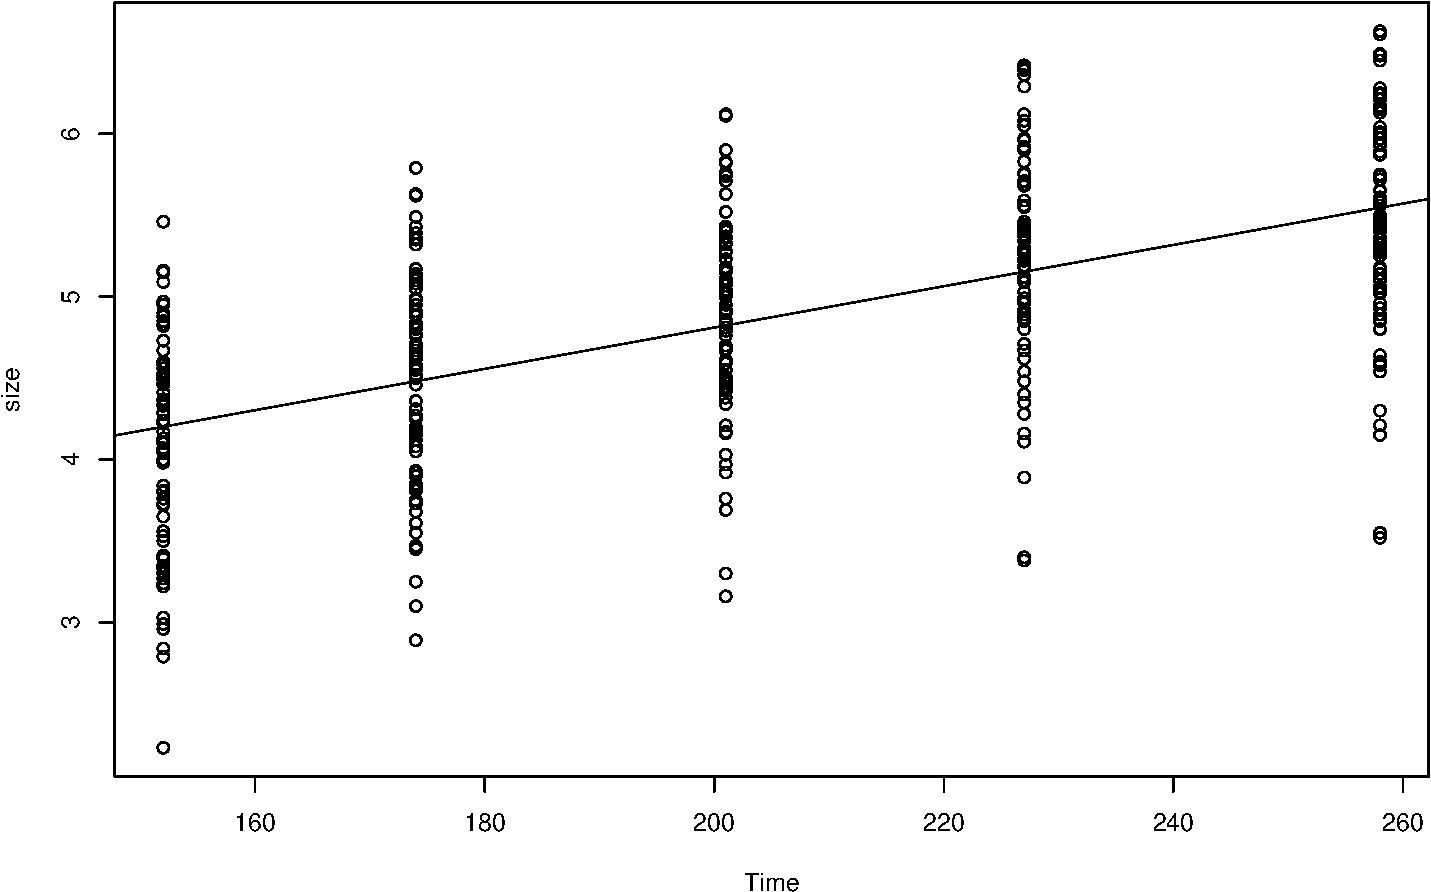
\includegraphics[height=0.7\textheight]{review_files/figure-beamer/unnamed-chunk-12-1}

\end{frame}

\end{document}
